%%
%% Copyright 2007, 2008, 2009 Elsevier Ltd
%%
%% This file is part of the 'Elsarticle Bundle'.
%% ---------------------------------------------
%%
%% It may be distributed under the conditions of the LaTeX Project Public
%% License, either version 1.2 of this license or (at your option) any
%% later version.  The latest version of this license is in
%%    http://www.latex-project.org/lppl.txt
%% and version 1.2 or later is part of all distributions of LaTeX
%% version 1999/12/01 or later.
%%
%% The list of all files belonging to the 'Elsarticle Bundle' is
%% given in the file `manifest.txt'.
%%

%% Template article for Elsevier's document class `elsarticle'
%% with numbered style bibliographic references
%% SP 2008/03/01

\documentclass[preprint,10pt,a4paper,5p,authoryear,twocolumn]{elsarticle}

%% Use the option review to obtain double line spacing
%% \documentclass[authoryear,preprint,review,12pt]{elsarticle}

%% Load custom macros
\usepackage{macros}

%% For including figures, graphicx.sty has been loaded in
%% elsarticle.cls. If you prefer to use the old commands
%% please give \usepackage{epsfig}

%% The amssymb package provides various useful mathematical symbols
\usepackage{amssymb}
%% The amsthm package provides extended theorem environments
%% \usepackage{amsthm}

%% The lineno packages adds line numbers. Start line numbering with
%% \begin{linenumbers}, end it with \end{linenumbers}. Or switch it on
%% for the whole article with \linenumbers.
%\usepackage{lineno}

%% Set the bibliography style to be apalike i.e. author, year citation
\bibliographystyle{apalike}
%% By default, elsarticle loads the natbib package with round parameter showing
%% round brackets in citations. This can be changed to sqaure by setting the
%% citestyle
\setcitestyle{square}

%% This turns references into clickable hyperlinks.
\usepackage[bookmarks,
            colorlinks=true,
            linkcolor=black,
            citecolor=black,
            urlcolor=blue,
            linktocpage,
            pageanchor=true]{hyperref} %,colorlinks

%% The subcaption package is used for figure and table sub-captions
\usepackage[list=true]{subcaption}

%% For code
\usepackage{listings}
\lstset{basicstyle=\scriptsize}

%% Journal
\journal{Computers \& Geosciences}

%% Setting the path to where the images can be found
\graphicspath{ {images/} }

%% Placeholder text
\usepackage{lipsum}

\begin{document}

\begin{frontmatter}
  \title{VTK in Climate Sciences}

\author[kitware]{Aashish Chaudhary}
\ead{aashish.chaudhary@kitware.com}

\author[kitware]{Sankhesh J. Jhaveri\corref{cor1}}
\ead{sankhesh.jhaveri@kitware.com}

\author[kitware]{Dan Lipsa\corref{}}
\ead{dan.lipsa@kitware.com}

\author[kitware]{David Lonie}
\ead{david.lonie@kitware.com}

\author[llnl]{Charles Doutriaux}
\ead{doutriaux1@llnl.gov}

\author[llnl]{Dean N. Williams}
\ead{Williams13@llnl.gov}

\address[kitware]{Kitware, Inc., 28 Corporate Drive, Clifton Park, NY 12065,
                  USA}
\address[llnl]{Lawrence Livermore National Laboratory, 7000 East Ave.,
               Livermore, CA 94550-9234}

\cortext[cor1]{Corresponding Author}


  \begin{abstract}
\label{abstract}
\lipsum[1]
\end{abstract}


  \begin{keyword}
    Visualization Toolkit \sep
    Climate data analysis \sep
    Scientific visualization \sep
    Climate visualization \sep
  \end{keyword}
\end{frontmatter}

\section{Introduction}
\label{introduction}
\begin{figure}[htb]
  \centering
  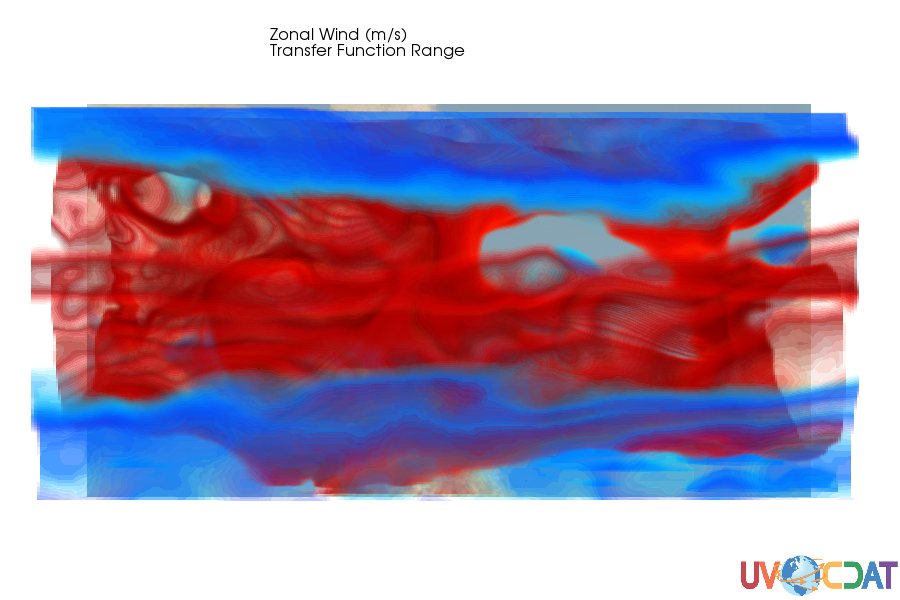
\includegraphics[width=\columnwidth]{dv3d_volume_test.png}
  \caption{Volume visualization using VTK in UV-CDAT}
  \label{fig:dv3d-volume}
\end{figure}[htb]
\lipsum*[1]~\citep{schroeder_visualization_2006}

\section{Approach}
\label{approach}
\lipsum*[1]

\section{Results}
\label{results}
\lipsum[2-3]

\section{Conclusion}
\label{conclusion}
\lipsum*[1]

\section{Acknowledgements}
\label{acknowledgements}
\lipsum*[4]


%% References:
\section{References}
\label{references}
\bibliography{VTKGeoSciences}

\end{document}
\endinput
%%
%% End of file `VTKGeoSciences.tex'.
